%
% ---------------------------------------------------------------
% Copyright (C) 2012-2018 Gang Li
% ---------------------------------------------------------------
%
% This work is the default powerdot-tuliplab style test file and may be
% distributed and/or modified under the conditions of the LaTeX Project Public
% License, either version 1.3 of this license or (at your option) any later
% version. The latest version of this license is in
% http://www.latex-project.org/lppl.txt and version 1.3 or later is part of all
% distributions of LaTeX version 2003/12/01 or later.
%
% This work has the LPPL maintenance status "maintained".
%
% This Current Maintainer of this work is Gang Li.
%
%

\documentclass[
 size=14pt,
 paper=smartboard,  %a4paper, smartboard, screen
 mode=present, 		%present, handout, print
 display=slides, 	% slidesnotes, notes, slides
 style=tuliplab,  	% TULIP Lab style
 pauseslide,
 fleqn,leqno]{powerdot}


\usepackage{cancel}
\usepackage{caption}
\usepackage{stackengine}
\usepackage{smartdiagram}
\usepackage{attrib}
\usepackage{amssymb}
\usepackage{amsmath}
\usepackage{amsthm}
\usepackage{mathtools}
\usepackage{rotating}
\usepackage{graphicx}
\usepackage{boxedminipage}
\usepackage{rotate}
\usepackage{calc}
\usepackage[absolute]{textpos}
\usepackage{psfrag,overpic}
\usepackage{fouriernc}
\usepackage{pstricks,pst-3d,pst-grad,pstricks-add,pst-text,pst-node,pst-tree}
\usepackage{moreverb,epsfig,subfigure}
\usepackage{color}
\usepackage{booktabs}
\usepackage{etex}
\usepackage{breqn}
\usepackage{multirow}
\usepackage{natbib}
\usepackage{bibentry}
\usepackage{gitinfo2}
\usepackage{siunitx}
\usepackage{nicefrac}
%\usepackage{geometry}
%\geometry{verbose,letterpaper}
\usepackage{media9}
\usepackage{animate}
%\usepackage{movie15}
\usepackage{auto-pst-pdf}

\usepackage{breakurl}
\usepackage{fontawesome}
\usepackage{xcolor}
\usepackage{multicol}



\usepackage{verbatim}
\usepackage[utf8]{inputenc}
\usepackage{dtk-logos}
\usepackage{tikz}
\usepackage{adigraph}
%\usepackage{tkz-graph}
\usepackage{hyperref}
%\usepackage{ulem}
\usepackage{pgfplots}
\usepackage{verbatim}
\usepackage{fontawesome}


\usepackage{todonotes}
% \usepackage{pst-rel-points}
\usepackage{animate}
\usepackage{fontawesome}

\usepackage{listings}
\lstset{frameround=fttt,
frame=trBL,
stringstyle=\ttfamily,
backgroundcolor=\color{yellow!20},
basicstyle=\footnotesize\ttfamily}
\lstnewenvironment{code}{
\lstset{frame=single,escapeinside=`',
backgroundcolor=\color{yellow!20},
basicstyle=\footnotesize\ttfamily}
}{}


\usepackage{hyperref}
\hypersetup{ % TODO: PDF meta Data
  pdftitle={Presentation Title},
  pdfauthor={Gang Li},
  pdfpagemode={FullScreen},
  pdfborder={0 0 0}
}


% \usepackage{auto-pst-pdf}
% package to show source code

\definecolor{LightGray}{rgb}{0.9,0.9,0.9}
\newlength{\pixel}\setlength\pixel{0.000714285714\slidewidth}
\setlength{\TPHorizModule}{\slidewidth}
\setlength{\TPVertModule}{\slideheight}
\newcommand\highlight[1]{\fbox{#1}}
\newcommand\icite[1]{{\footnotesize [#1]}}

\newcommand\twotonebox[2]{\fcolorbox{pdcolor2}{pdcolor2}
{#1\vphantom{#2}}\fcolorbox{pdcolor2}{white}{#2\vphantom{#1}}}
\newcommand\twotoneboxo[2]{\fcolorbox{pdcolor2}{pdcolor2}
{#1}\fcolorbox{pdcolor2}{white}{#2}}
\newcommand\vpspace[1]{\vphantom{\vspace{#1}}}
\newcommand\hpspace[1]{\hphantom{\hspace{#1}}}
\newcommand\COMMENT[1]{}

\newcommand\placepos[3]{\hbox to\z@{\kern#1
        \raisebox{-#2}[\z@][\z@]{#3}\hss}\ignorespaces}

\renewcommand{\baselinestretch}{1.2}


\newcommand{\draftnote}[3]{
	\todo[author=#2,color=#1!30,size=\footnotesize]{\textsf{#3}}	}
% TODO: add yourself here:
%
\newcommand{\gangli}[1]{\draftnote{blue}{GLi:}{#1}}
\newcommand{\shaoni}[1]{\draftnote{green}{sn:}{#1}}
\newcommand{\gliMarker}
	{\todo[author=GLi,size=\tiny,inline,color=blue!40]
	{Gang Li has worked up to here.}}
\newcommand{\snMarker}
	{\todo[author=Sn,size=\tiny,inline,color=green!40]
	{Shaoni has worked up to here.}}

%%%%%%%%%%%%%%%%%%%%%%%%%%%%%%%%%%%%%%%%%%%%%%%%%%%%%%%%%%%%%%%%%%%%%%%%
% title
% TODO: Customize to your Own Title, Name, Address
%
\title{Flip 00 Project Report}
\author{
Jing Miao
\\
\\Qingdao University of Technology
}
\date{October 16th}


% Customize the setting of slides
\pdsetup{
% TODO: Customize the left footer, and right footer
rf=\href{http://www.tulip.org.au}{
Last Changed by: \textsc{\gitCommitterName}\ \gitVtagn-\gitAbbrevHash\ (\gitAuthorDate)
},
cf={Flip 00 Project Report},
}


\begin{document}

\maketitle

%\begin{slide}{Overview}
%\tableofcontents[content=sections]
%\end{slide}


%%==========================================================================================
%%
\begin{slide}[toc=,bm=]{Overview}
\tableofcontents[content=currentsection,type=1]
\end{slide}
%%
%%==========================================================================================


\section{Introduction}


%%==========================================================================================
%%
\begin{slide}{Project Introduction}
\begin{center}
\twotonebox{\rotatebox{90}{Defn}}{\parbox{.86\textwidth}
{This is about analyzing the factors that affect the usage of shared bicycles.
 Bike sharing is a way to rent bicycles,
 in which the process of obtaining membership,
 renting and returning the bicycle is automatically completed through a 
 network of stations in the city.
 Through the system,
 people can rent bicycles according to their needs,
 rent bicycles from a location,
 and then ride to the destination to return.
 This project analyzes the data used in historical weather to predict the
 rental demand of shared bicycles in the future.
}}
\end{center}


%%==========================================================================================

%%==========================================================================================

\end{slide}
%%
%%==========================================================================================
\section{Data Analysis}

%%==========================================================================================



\begin{slide}[toc=,bm=]{Statistical Analysis Data}
\begin{table}[tb]
\setlength{\abovecaptionskip}{0pt}
\setlength{\tabcolsep}{2pt}
\centering
\caption{Train Data Describe}
\scalebox{0.8}{
\begin{tabular}{c| c c c c c c c c c c c}
\toprule
%\centering
Attributes& \texttt{season}  & \texttt{holiday} & \texttt{workingday} & \texttt{weather}
       & \texttt{temp}  & \texttt{atemp} & \texttt{humidity} & \texttt{windspeed}
       & \texttt{casual} & \texttt{registered} & \texttt{count} \\
\midrule
$count$
&  {$10886$} &  {$10886$} &  {$10886$} &  {$10886$}
&  {$10886$} &  {$10886$} &  {$10886$} &  {$10886$}
&  {$10886$} &  {$10886$} &  {$10886$}\\
$mean$
&  {$2$} &  {$0$}&  {$0$}&  {$1$}
&  {$20$} &  {$23$}&  {$61$}&  {$12$}
&  {$36$} &  {$155$}&  {$191$}\\
$std$
&  {$1$}	&  {$0$}	&  {$0$}	&  {$0$}	
&  {$7$}	&  {$8$}	&  {$19$}	&  {$8$}	
&  {$49$}	&  {$151$}	&  {$181$} \\
$min$
&  {$1$}	&  {$0$}	&  {$0$}	&  {$1$}	
&  {$0$}	&  {$0$}	&  {$0$}	&  {$0$}	
&  {$0$}	&  {$0$}	&  {$1$} \\
$25\%$
&  {$2$}	&  {$0$}	&  {$0$}	&  {$1$}	
&  {$13$}	&  {$16$}	&  {$47$}	&  {$7$}	
&  {$4$}	&  {$36$}	&  {$42$} \\
$50\%$
&  {$3$}	&  {$0$}	&  {$1$}	&  {$1$}	
&  {$20$}	&  {$24$}	&  {$62$}	&  {$12$}	
&  {$17$}	&  {$118$}	&  {$145$} \\
$75\%$
&  {$4$}	&  {$0$}	&  {$1$}	&  {$2$}	
&  {$26$}	&  {$31$}	&  {$77$}	&  {$16$}	
&  {$49$}	&  {$222$}	&  {$284$} \\
$max$
&  {$4$}	&  {$1$}	&  {$1$}	&  {$4$}	
&  {$41$}	&  {$45$}	&  {$100$}	&  {$56$}	
&  {$367$}	&  {$886$}	&  {$977$} \\
\bottomrule
\end{tabular}
}
\end{table}
\end{slide}

%%==========================================================================================

\begin{slide}[toc=,bm=]{Statistical Analysis Data}
\begin{table}[tb]
\setlength{\abovecaptionskip}{0pt}
\setlength{\belowcaptionskip}{10pt}
\centering
\caption{Test Data Describe}
\scalebox{0.9}{
\begin{tabular}{c| c c c c c c c c}
\toprule
%\centering
Attributes& \texttt{season}  & \texttt{holiday} & \texttt{workingday} & \texttt{weather}
       & \texttt{temp}  & \texttt{atemp} & \texttt{humidity} & \texttt{windspeed} \\
\midrule
$count$
&  {$6493$}	&  {$6493$}	&  {$6493$}	&  {$6493$}	
&  {$6493$}	&  {$6493$}	&  {$6493$}	&  {$6493$}\\
$mean$
&  {$2$}	&  {$0$}	&  {$0$}	&  {$1$}	
&  {$20$}	&  {$24$}	&  {$64$}	&  {$12$}\\
$std$
&  {$1$}	&  {$0$}	&  {$0$}	&  {$0$}	
&  {$8$}	&  {$8$}	&  {$19$}	&  {$8$}\\
$min$	
&  {$1$}	&  {$0$}	&  {$0$}	&  {$1$}	
&  {$0$}	&  {$0$}	&  {$16$}	&  {$0$}\\
$25\%$	
&  {$2$}	&  {$0$}	&  {$0$}	&  {$1$}	
&  {$13$}	&  {$16$}	&  {$49$}	&  {$7$}\\
$50\%$	
&  {$3$}	&  {$0$}	&  {$1$}	&  {$1$}	
&  {$21$}	&  {$25$}	&  {$65$}	&  {$11$}\\
$75\%$	
&  {$3$}	&  {$0$}	&  {$1$}	&  {$2$}	
&  {$27$}	&  {$31$}	&  {$81$}	&  {$16$}\\
$max$	
&  {$4$}	&  {$1$}	&  {$1$}	&  {$4$}
&  {$40$}	&  {$50$}	&  {$100$}	&  {$55$}\\
\bottomrule
\end{tabular}
}
\end{table}
\end{slide}
%%
%%==========================================================================================
\begin{slide}[toc=,bm=]{Statistical Analysis Data}
\begin{table}[tb]
\setlength{\abovecaptionskip}{0pt}
\setlength{\belowcaptionskip}{10pt}
\centering
\caption{The first Two Rows of The Train Data}
\scalebox{0.6}{
\begin{tabular}{c| c c c c c c c c c c c c}
\toprule
%\centering
   & \texttt{datetime} & \texttt{season}  & \texttt{holiday}
& \texttt{workingday} & \texttt{weather} & \texttt{temp}  & \texttt{atemp}
& \texttt{humidity}   & \texttt{windspeed} & \texttt{casual} & \texttt{registered}
& \texttt{count}\\
\midrule
$0$
&  {$2011-01-01 00:00:00$}	&  {$1$}	&  {$0$}	&  {$0$}	
&  {$1$}	&  {$9.84$}&  {$14.395$}	&  {$81$}  &  {$0.0$}
&  {$3$}	&  {$13$}  &  {$16$}\\
$1$
&  {$2011-01-01 01:00:00$}	&  {$1$}	&  {$0$}	&  {$0$}	
&  {$1$}	&  {$9.02$}&  {$13.635$}	&  {$80$}  &  {$0.0$}
&  {$8$}	&  {$32$}  &  {$40$}\\
\bottomrule
\end{tabular}
}
\end{table}
{Conclusion
\begin{itemize}
\item
\smallskip
%It can be seen from the scalar type that it is basically divided into two categories: time and weather.
By viewing variable data type,the columns "season","holiday","workingday" and "weather" should be of "categorical" data type.But the current data type is "int" for those columns.So to transform the dataset in the following ways so that we can get started up with our EDA.
\smallskip
\item
\smallskip
Luckily we don't have any missing value in the dataset.
\end{itemize}
}
\end{slide}


%%==========================================================================================
%%==========================================================================================

\begin{slide}[toc=,bm=]{Outliers Analysis}
\begin{itemize}
\item
The "count","season","hour","workingday" variable Boxplot
\end{itemize}
\vspace{-0.8cm}
\begin{center}
  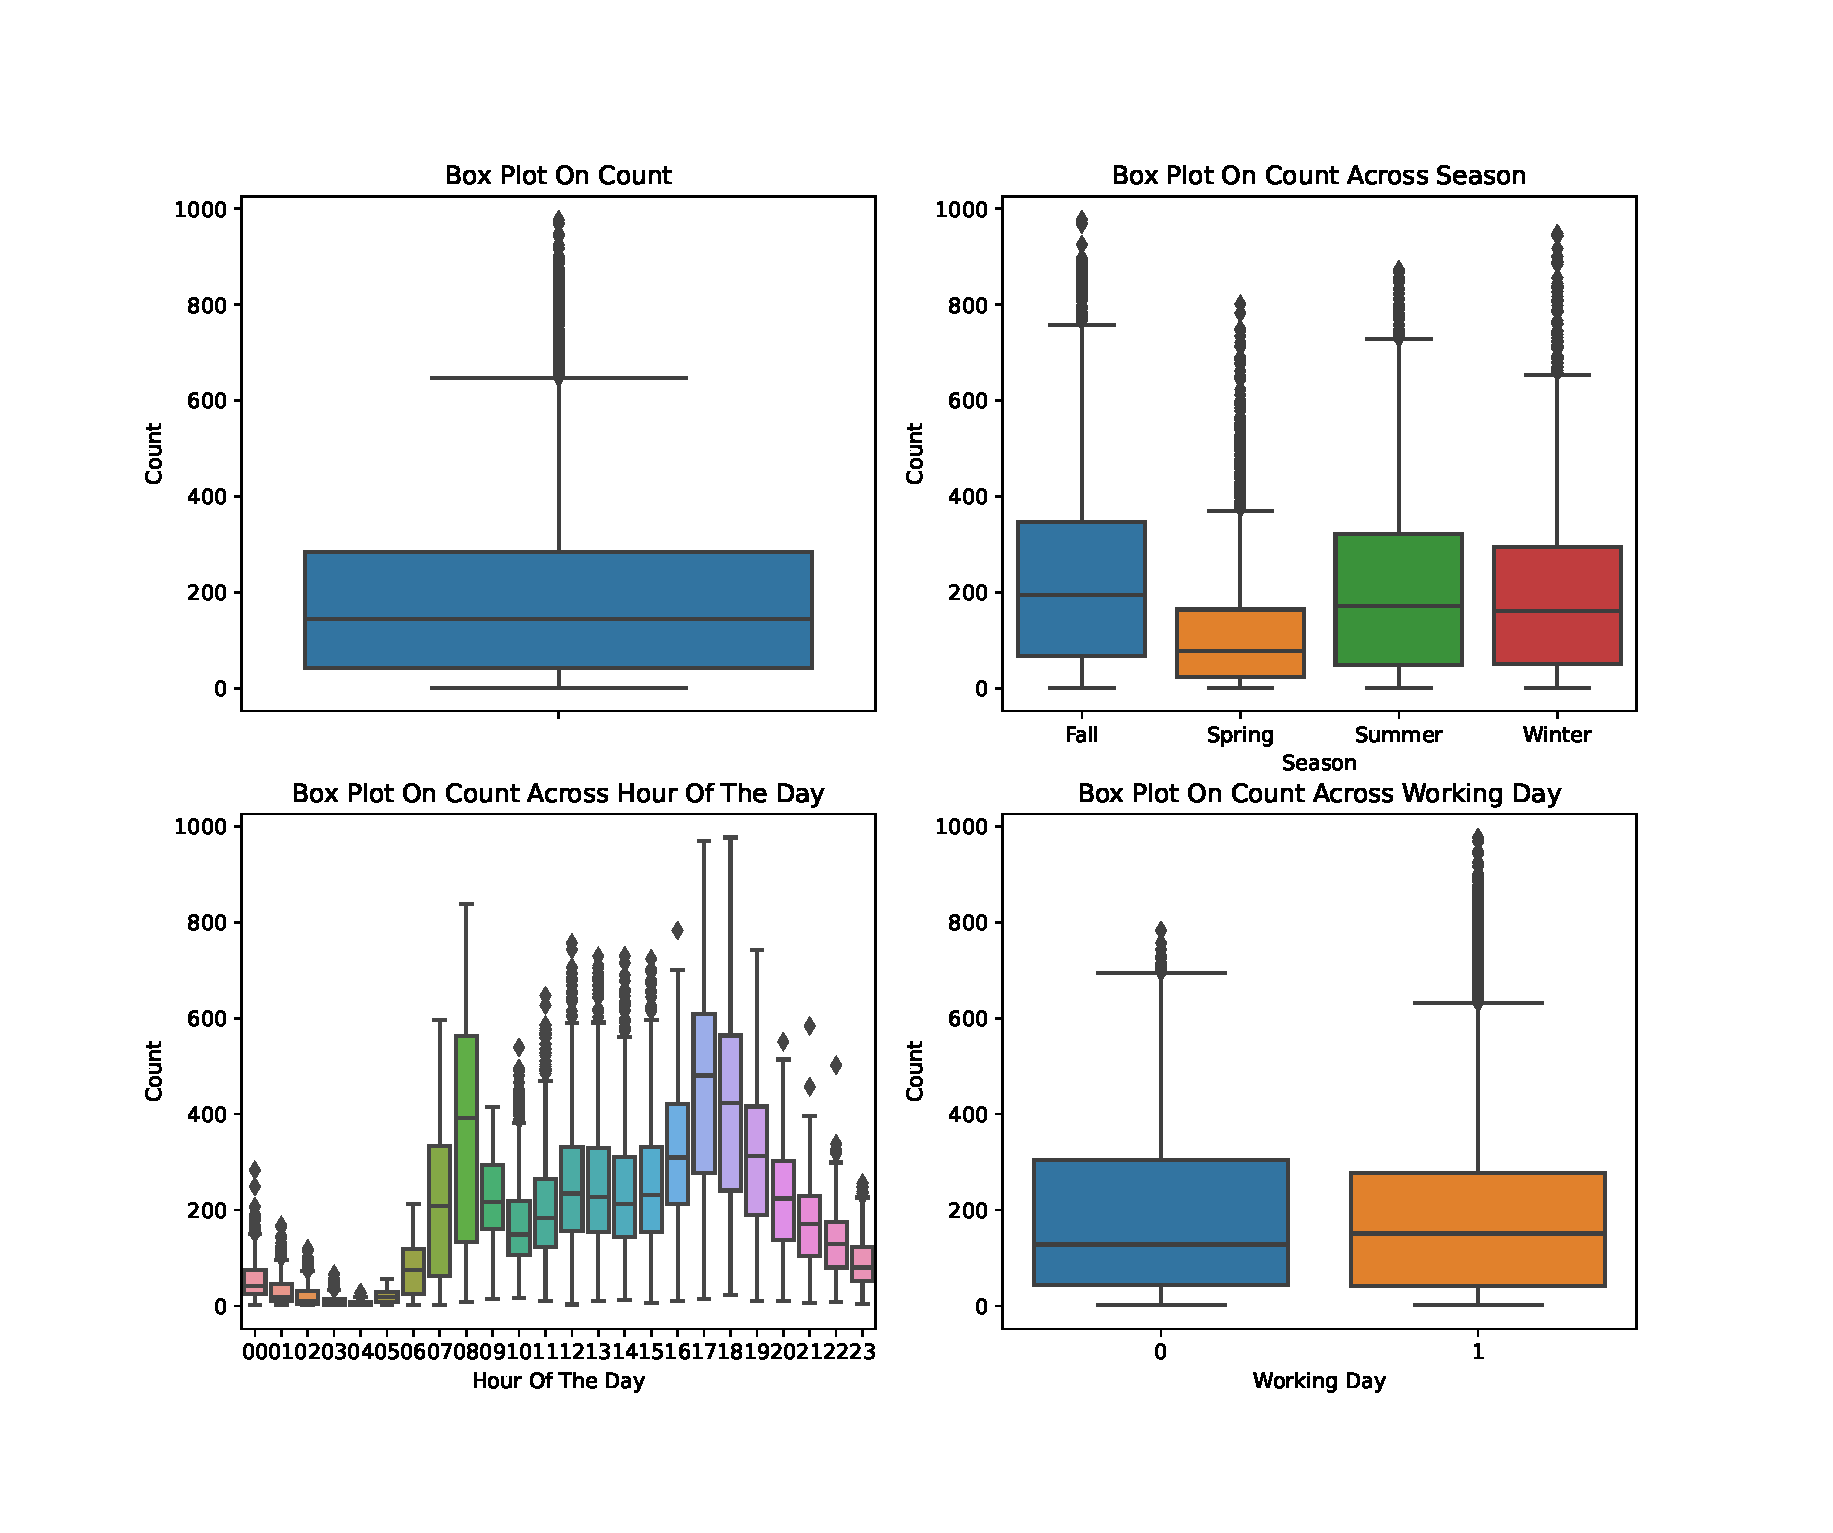
\includegraphics[width=.9\linewidth,height=.5\linewidth]{C:/FILP00report/picture/hour.eps}
\end{center}
\end{slide}

%%==========================================================================================
\begin{slide}{Outliers Analysis Conclusion}
\begin{itemize}
\item
At first look, "count" variable contains lot of outlier data points which skews the distribution towards right (as there are more data points beyond Outer Quartile Limit).But in addition to that, following inferences can also been made from the simple boxplots given below.
\item
Spring season has got relatively lower count.The dip in median value in boxplot gives evidence for it.
\item
The boxplot with "Hour Of The Day" is quiet interesting.The median value are relatively higher at 7AM - 8AM and 5PM - 6PM. It can be attributed to regular school and office users at that time.
\item
Most of the outlier points are mainly contributed from "Working Day" than "Non Working Day". It is quiet visible from from figure 4.
\end{itemize}
\end{slide}

%%==========================================================================================

\begin{slide}[toc=,bm=]{Correlation Analysis}
\begin{itemize}
\item
Plot a correlation plot between "count" \& "temp","atemp","humidity","windspeed"
\end{itemize}
\vspace{-1.0cm}

\begin{figure}
  \centering
  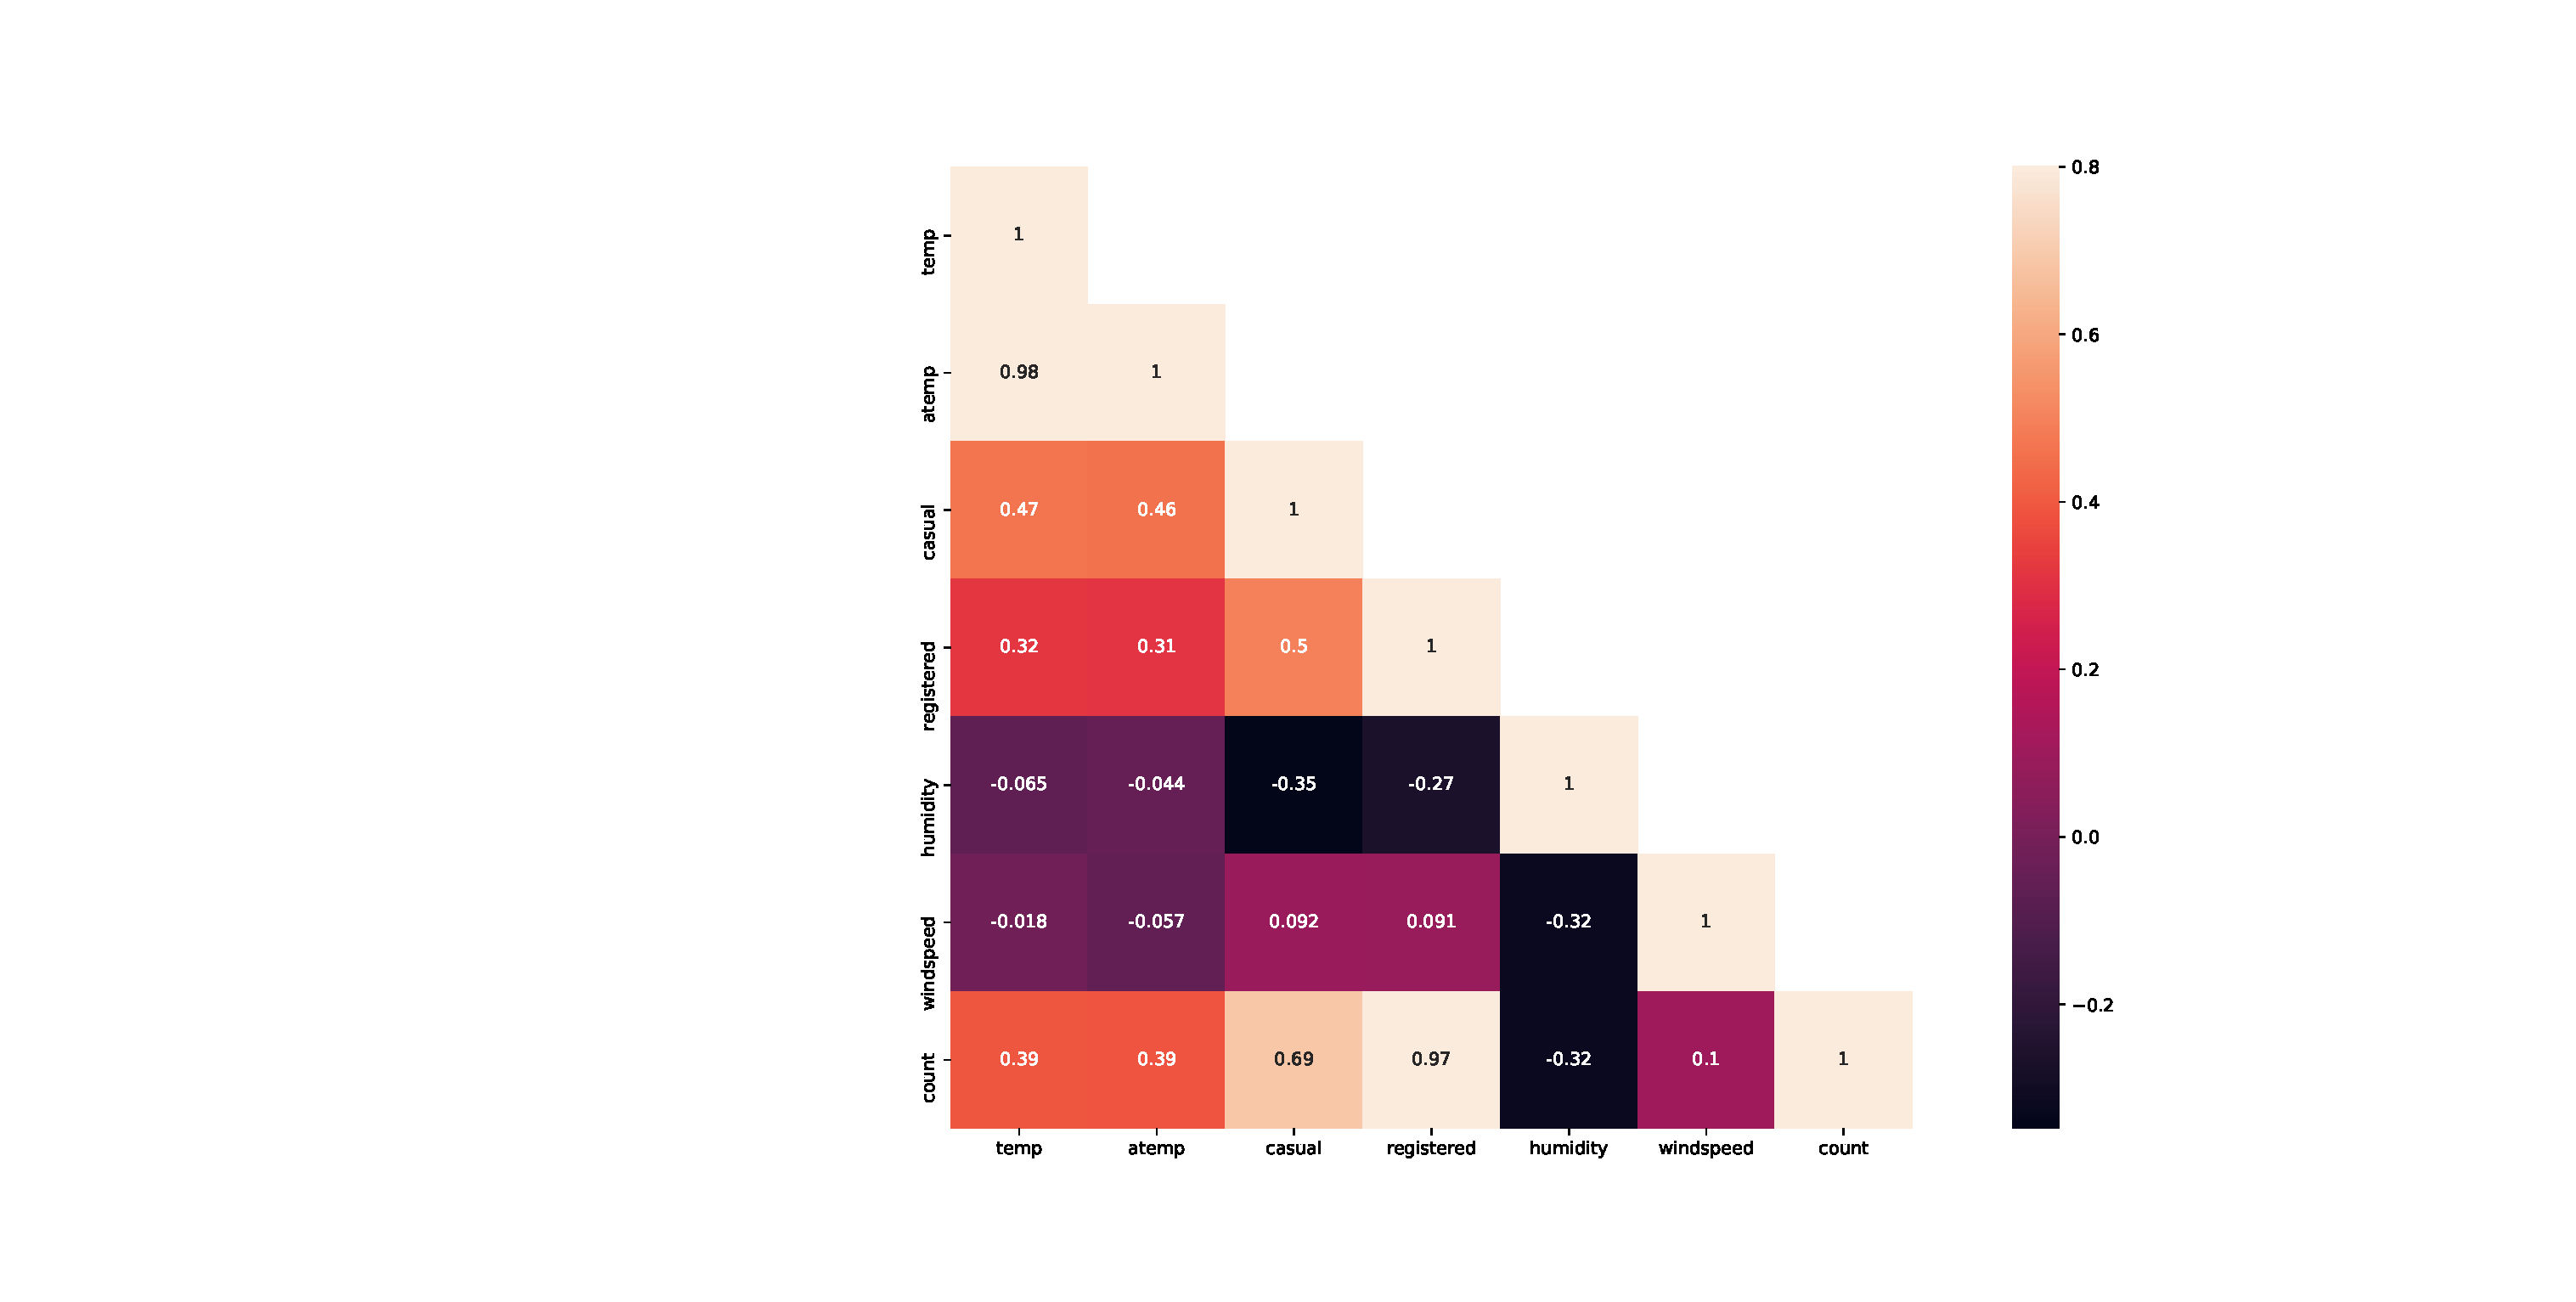
\includegraphics[width=1.0\linewidth,height=.5\linewidth]{C:/FILP00report/picture/AxesSubplots.eps}

\end{figure}

\end{slide}
\begin{slide}{Correlation Analysis Conclusion}
\begin{itemize}
\item
Temp and humidity features has got positive and negative correlation with count respectively.Although the correlation between them are not very prominent still the count variable has got little dependency on "temp" and "humidity".
\item
Windspeed is not gonna be really useful numerical feature and it is visible from it correlation value with "count"
\item
"atemp" is variable is not taken into since "atemp" and "temp" has got strong correlation with each other. During model building any one of the variable has to be dropped since they will exhibit multicollinearity in the data.
\item
"Casual" and "Registered" are also not taken into account since they are leakage variables in nature and need to dropped during model building.
\end{itemize}
\end{slide}
%%==========================================================================================
%%==========================================================================================

\section{Feature Engineering}
\begin{slide}[toc=,bm=]{Skewness In Distribution}
\begin{itemize}
\item
Create new columns "date,"hour","weekDay","month" from "datetime" column.
Coerce the datatype of "season","holiday","workingday" and weather to category.
Drop the datetime column as we already extracted useful features from it.
\end{itemize}
\begin{center}
  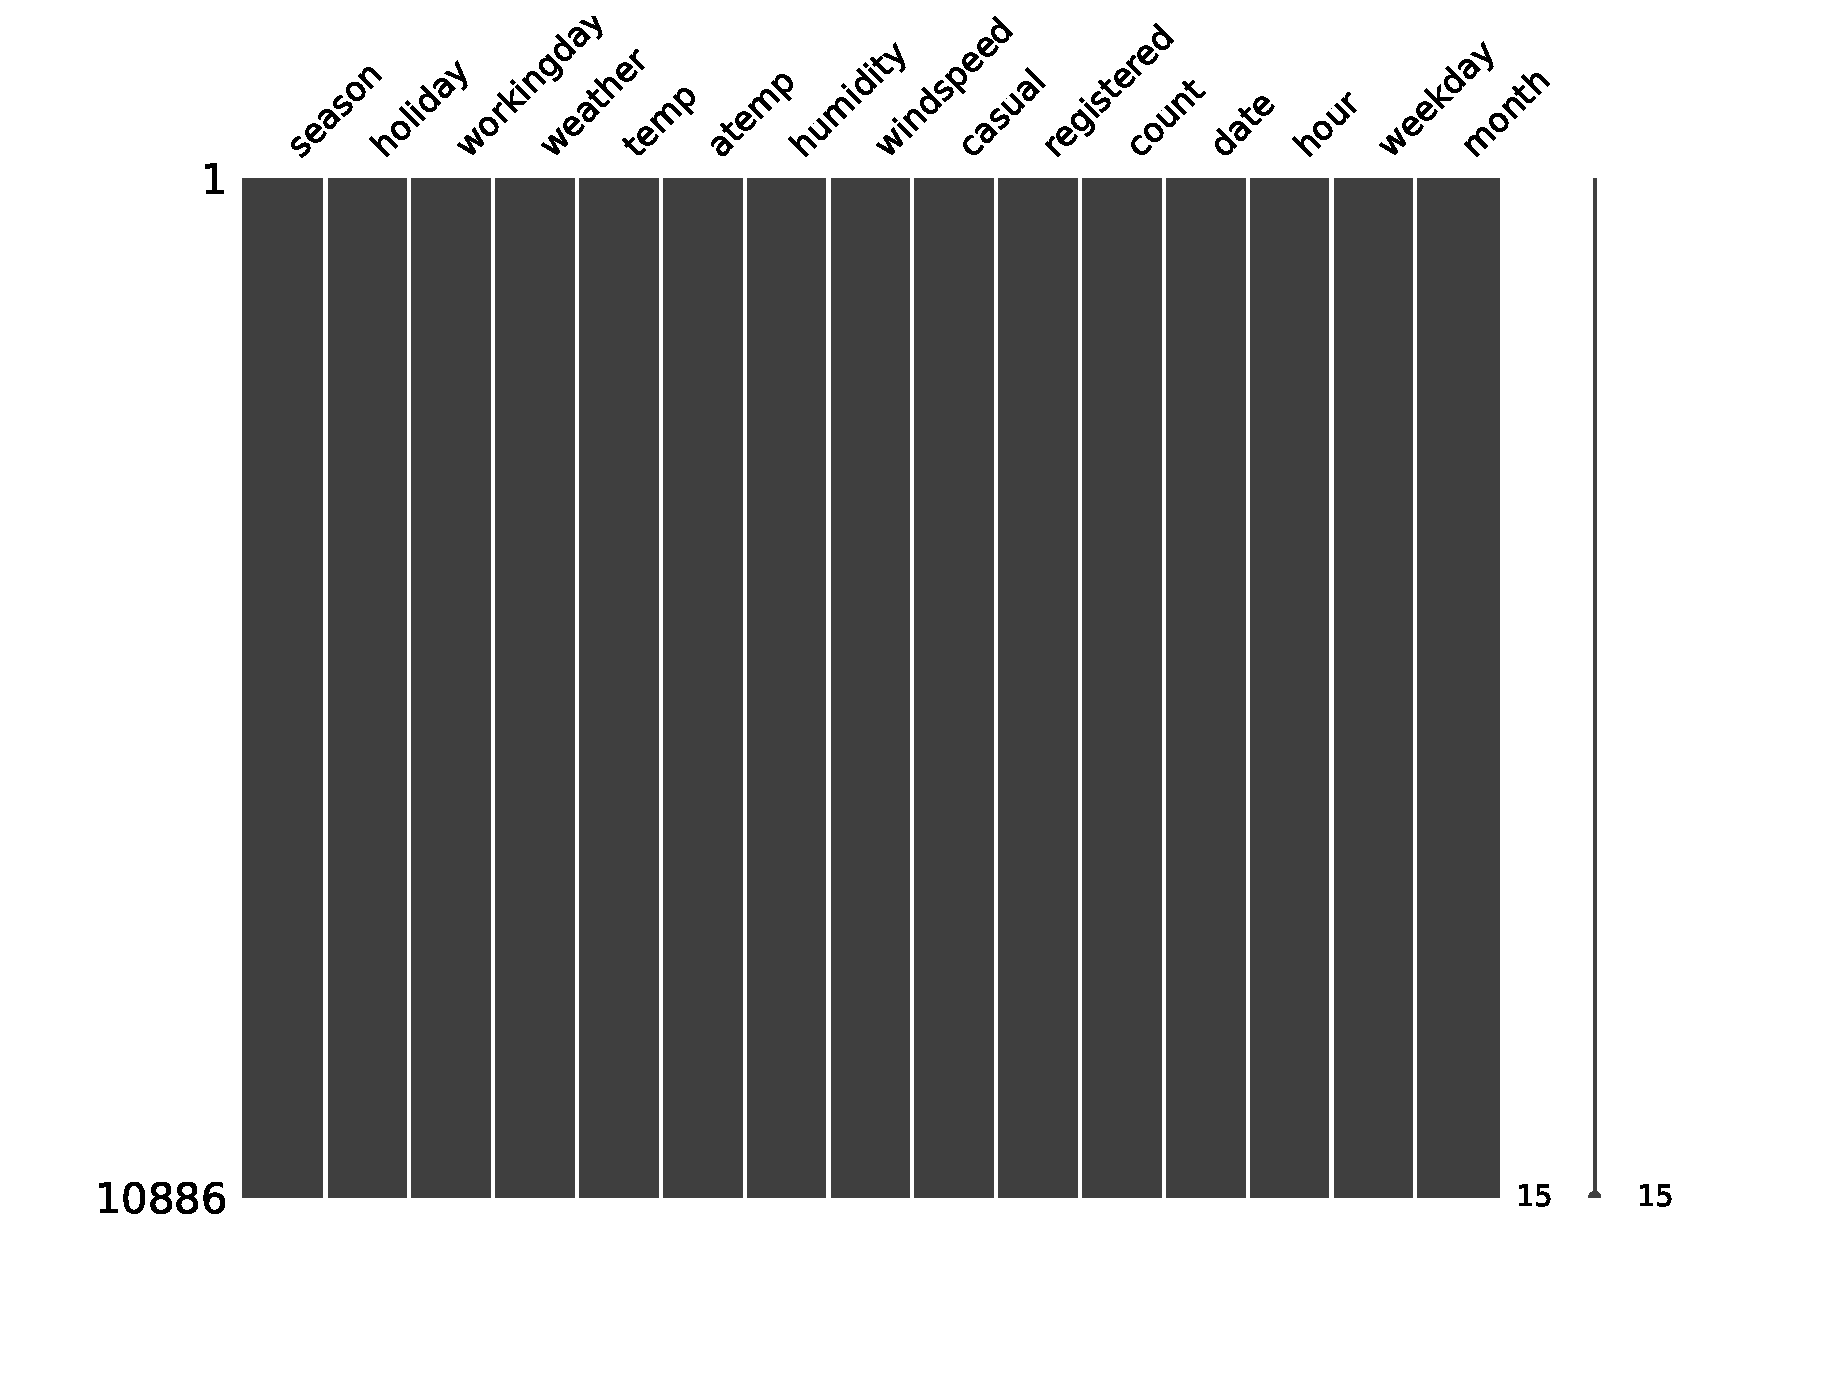
\includegraphics[width=.8\linewidth,height=.4\linewidth]{C:/FILP00report/picture/axes.eps}
\end{center}
\end{slide}

%%==========================================================================================

\begin{slide}[toc=,bm=]{Fill in outliers}
\begin{itemize}
\item
Filling 0's In Windspeed Before Using Random Forest
\end{itemize}
\begin{center}
  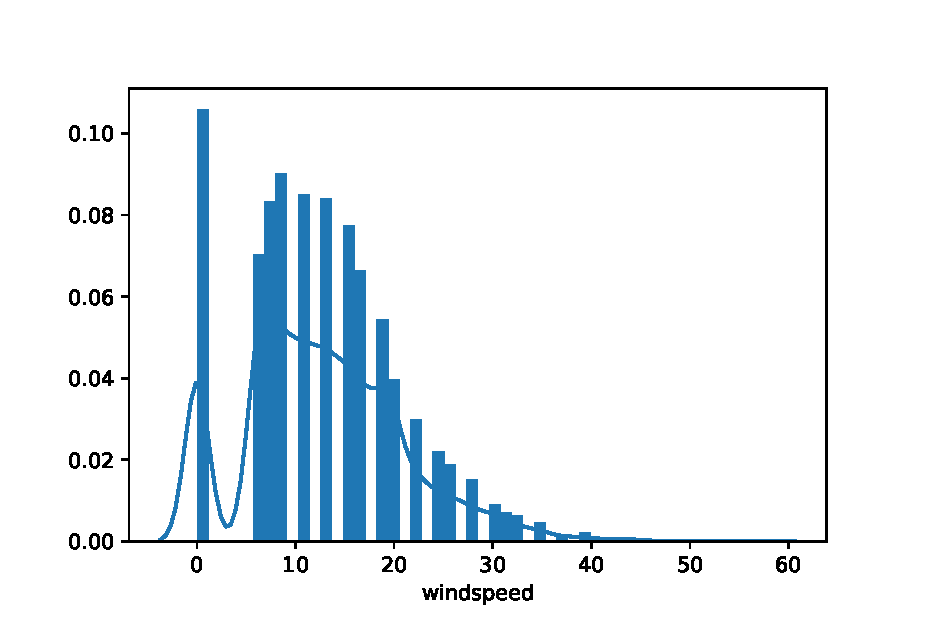
\includegraphics[width=.8\linewidth,height=.4\linewidth]{C:/FILP00report/picture/windspeedpre.eps}
\end{center}
\end{slide}
%%==========================================================================================
\begin{slide}[toc=,bm=]{Fill in outliers}
\begin{itemize}
\item
Filling 0's In Windspeed After Using Random Forest
\end{itemize}
\begin{center}
  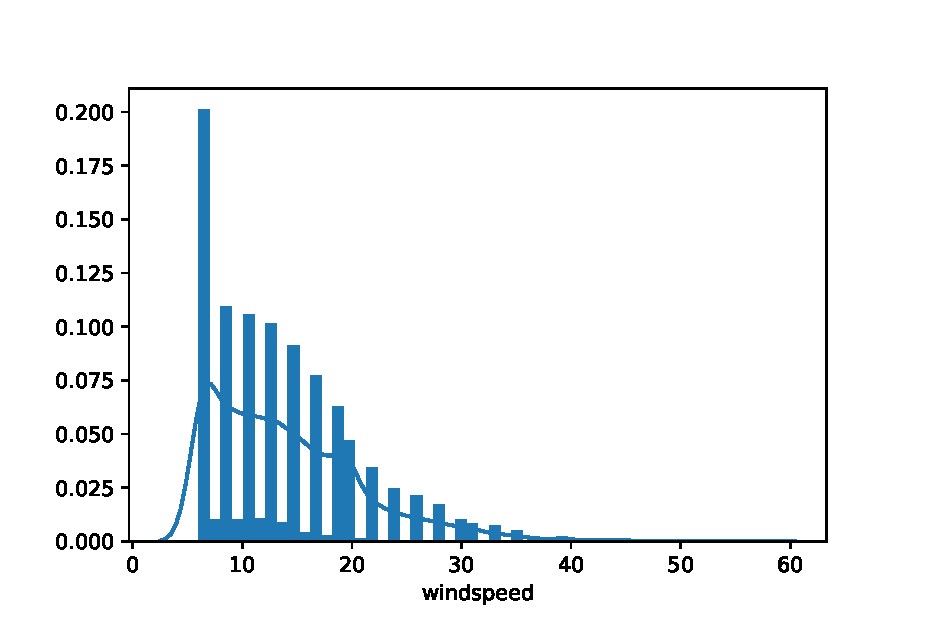
\includegraphics[width=.8\linewidth,height=.4\linewidth]{C:/FILP00report/picture/windspeedaft.eps}
\end{center}
\end{slide}
%%==========================================================================================

\section{Data Visualization}

%%==========================================================================================

\begin{slide}[toc=,bm=]{Visualizing Distribution Of Data}
\begin{itemize}
\item
Draw density graph to view the count column data
\end{itemize}
\begin{center}
  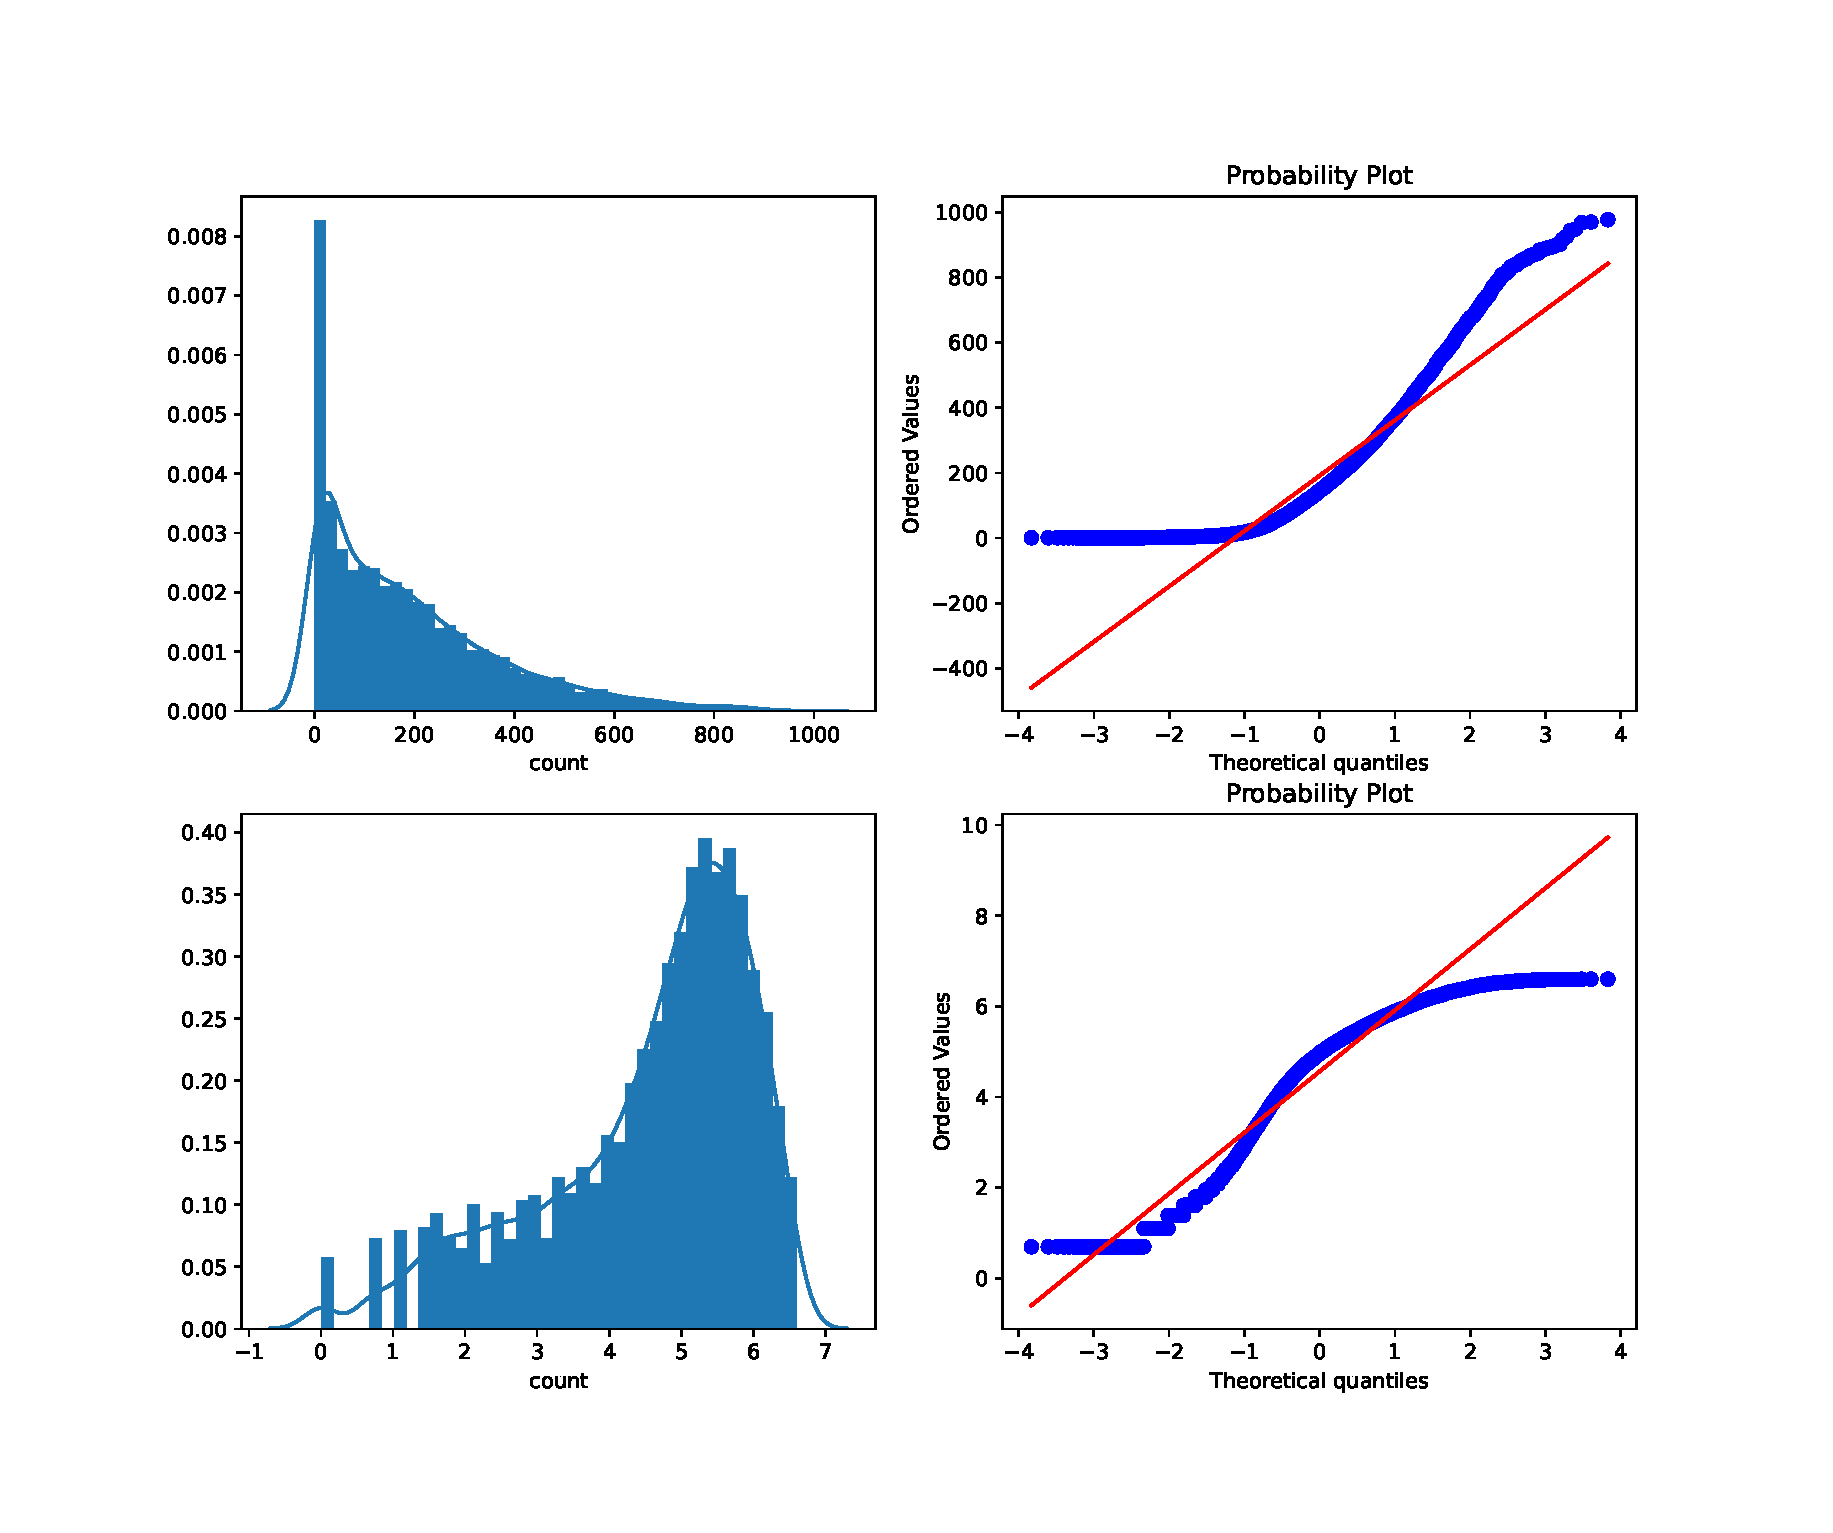
\includegraphics[width=.9\linewidth,height=.5\linewidth]{C:/FILP00report/picture/keshihuafb.eps}
\end{center}
\end{slide}

%%==========================================================================================

\begin{slide}{Visualizing Distribution Of Data}
\begin{itemize}
\item
As it is visible from the below figures that "count" variable is skewed towards right. It is desirable to have Normal distribution as most of the machine learning techniques require dependent variable to be Normal.
\item
 One possible solution is to take log transformation on "count" variable after removing outlier data points. After the transformation the data looks lot better but still not ideally following normal distribution.
\end{itemize}
\end{slide}


%%==========================================================================================

%%==========================================================================================
%%
\begin{slide}[toc=,bm=]{Visualizing Count Vs (Month,Season)}
\begin{itemize}
\item
Month \& Season
\end{itemize}
\vspace{-0.8cm}
\begin{center}
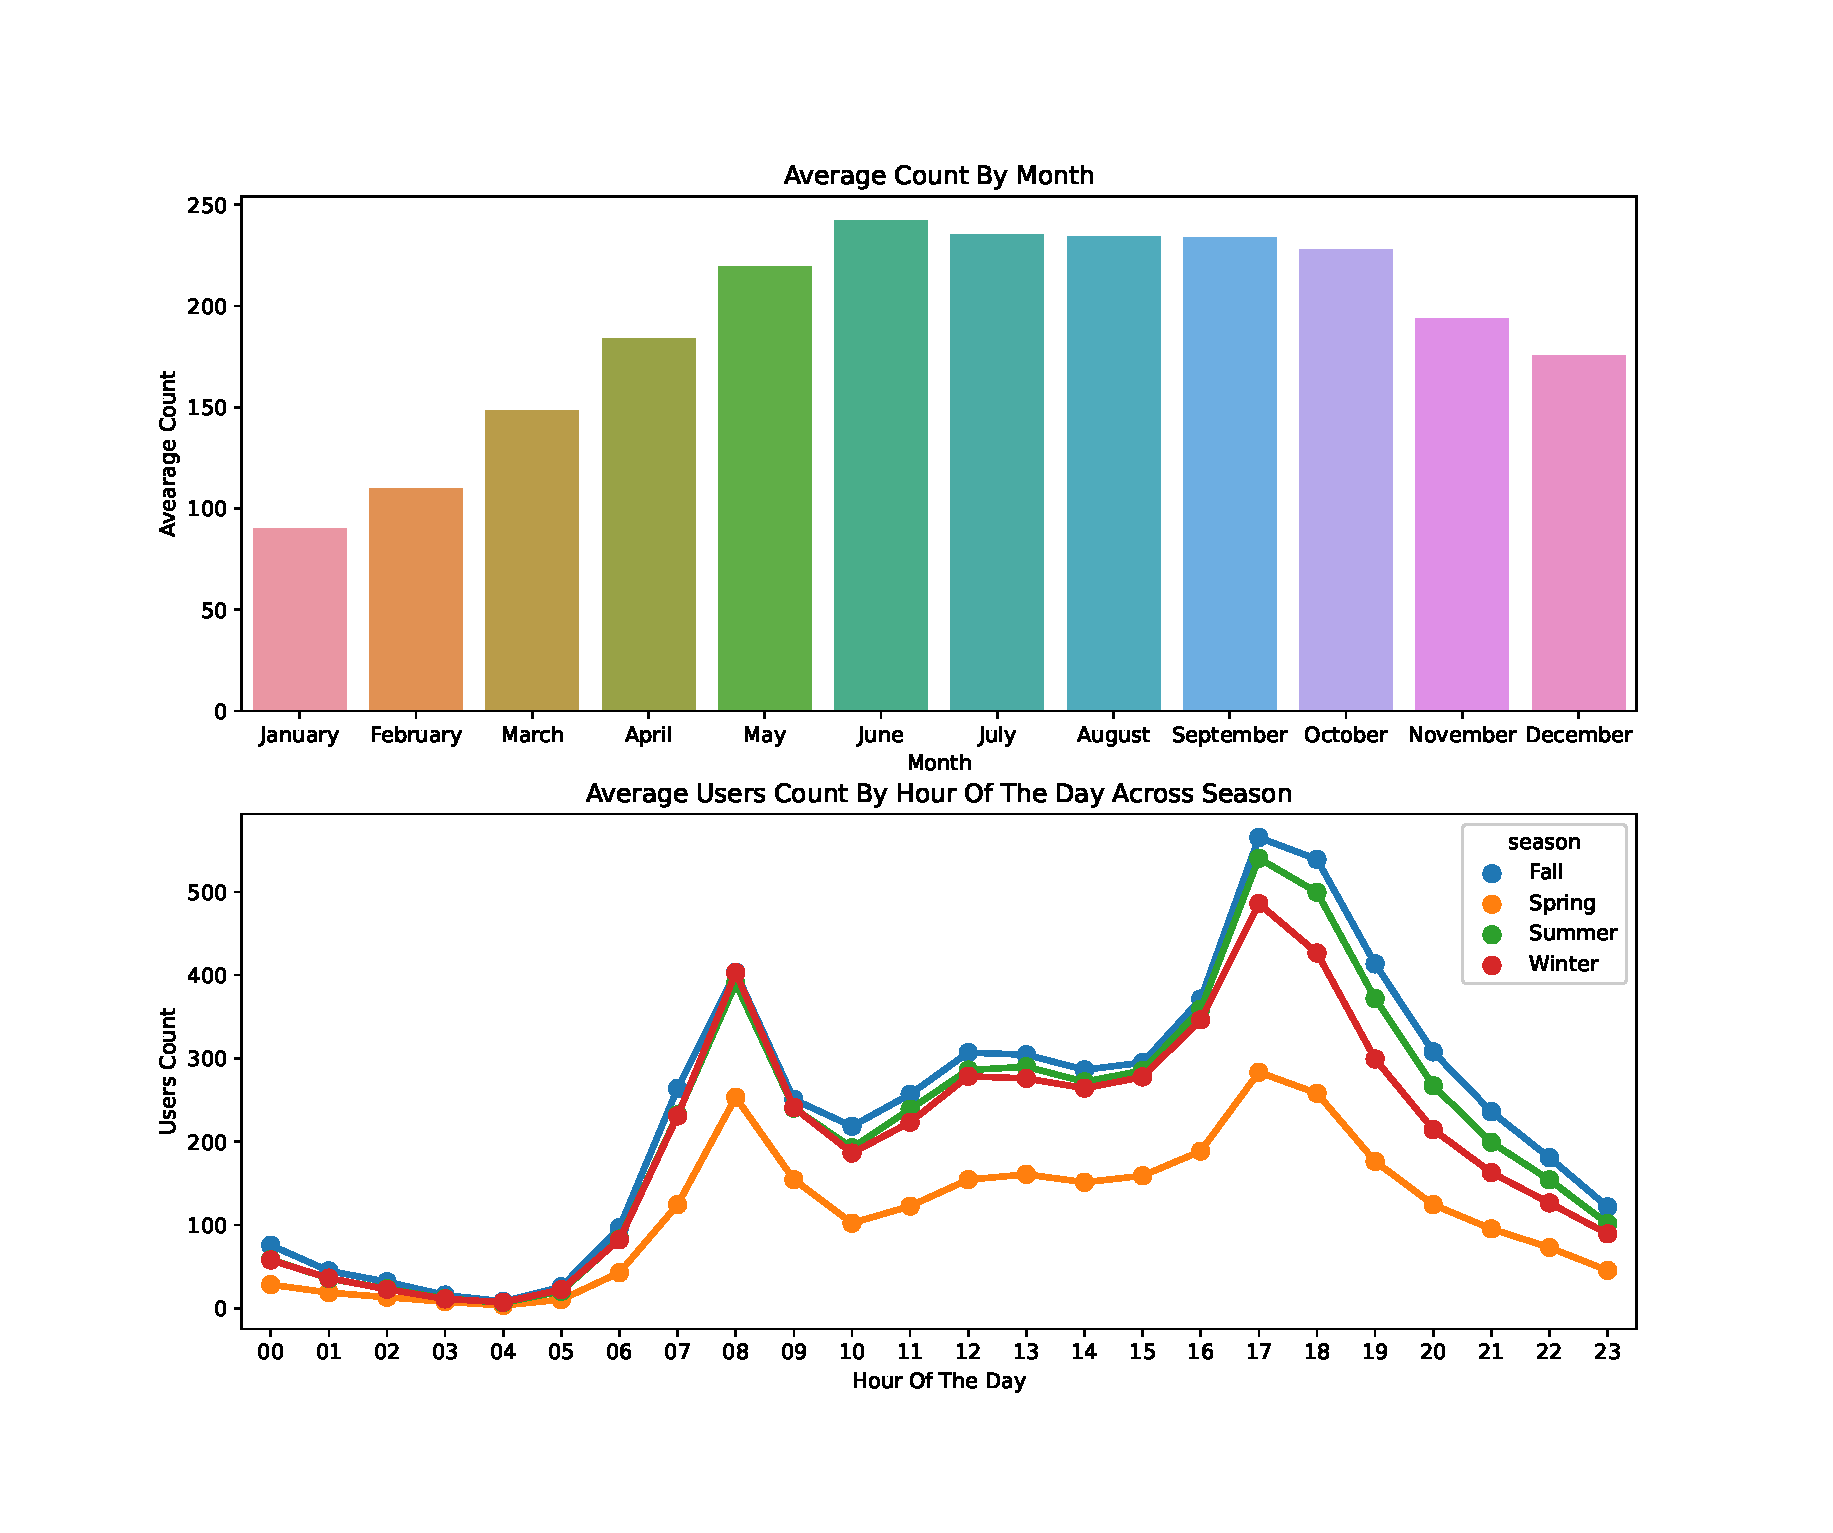
\includegraphics[width=.8\linewidth,height=.55\linewidth]{C:/FILP00report/picture/keshihua1.eps}
\end{center}
\end{slide}

%%==========================================================================================


\begin{slide}[toc=,bm=]{Visualizing Count Vs (Hour,Weekday,Usertype)}
\begin{itemize}
\item
Hour,Weekday \& Usertype
\end{itemize}
\vspace{-0.8cm}
\begin{center}
  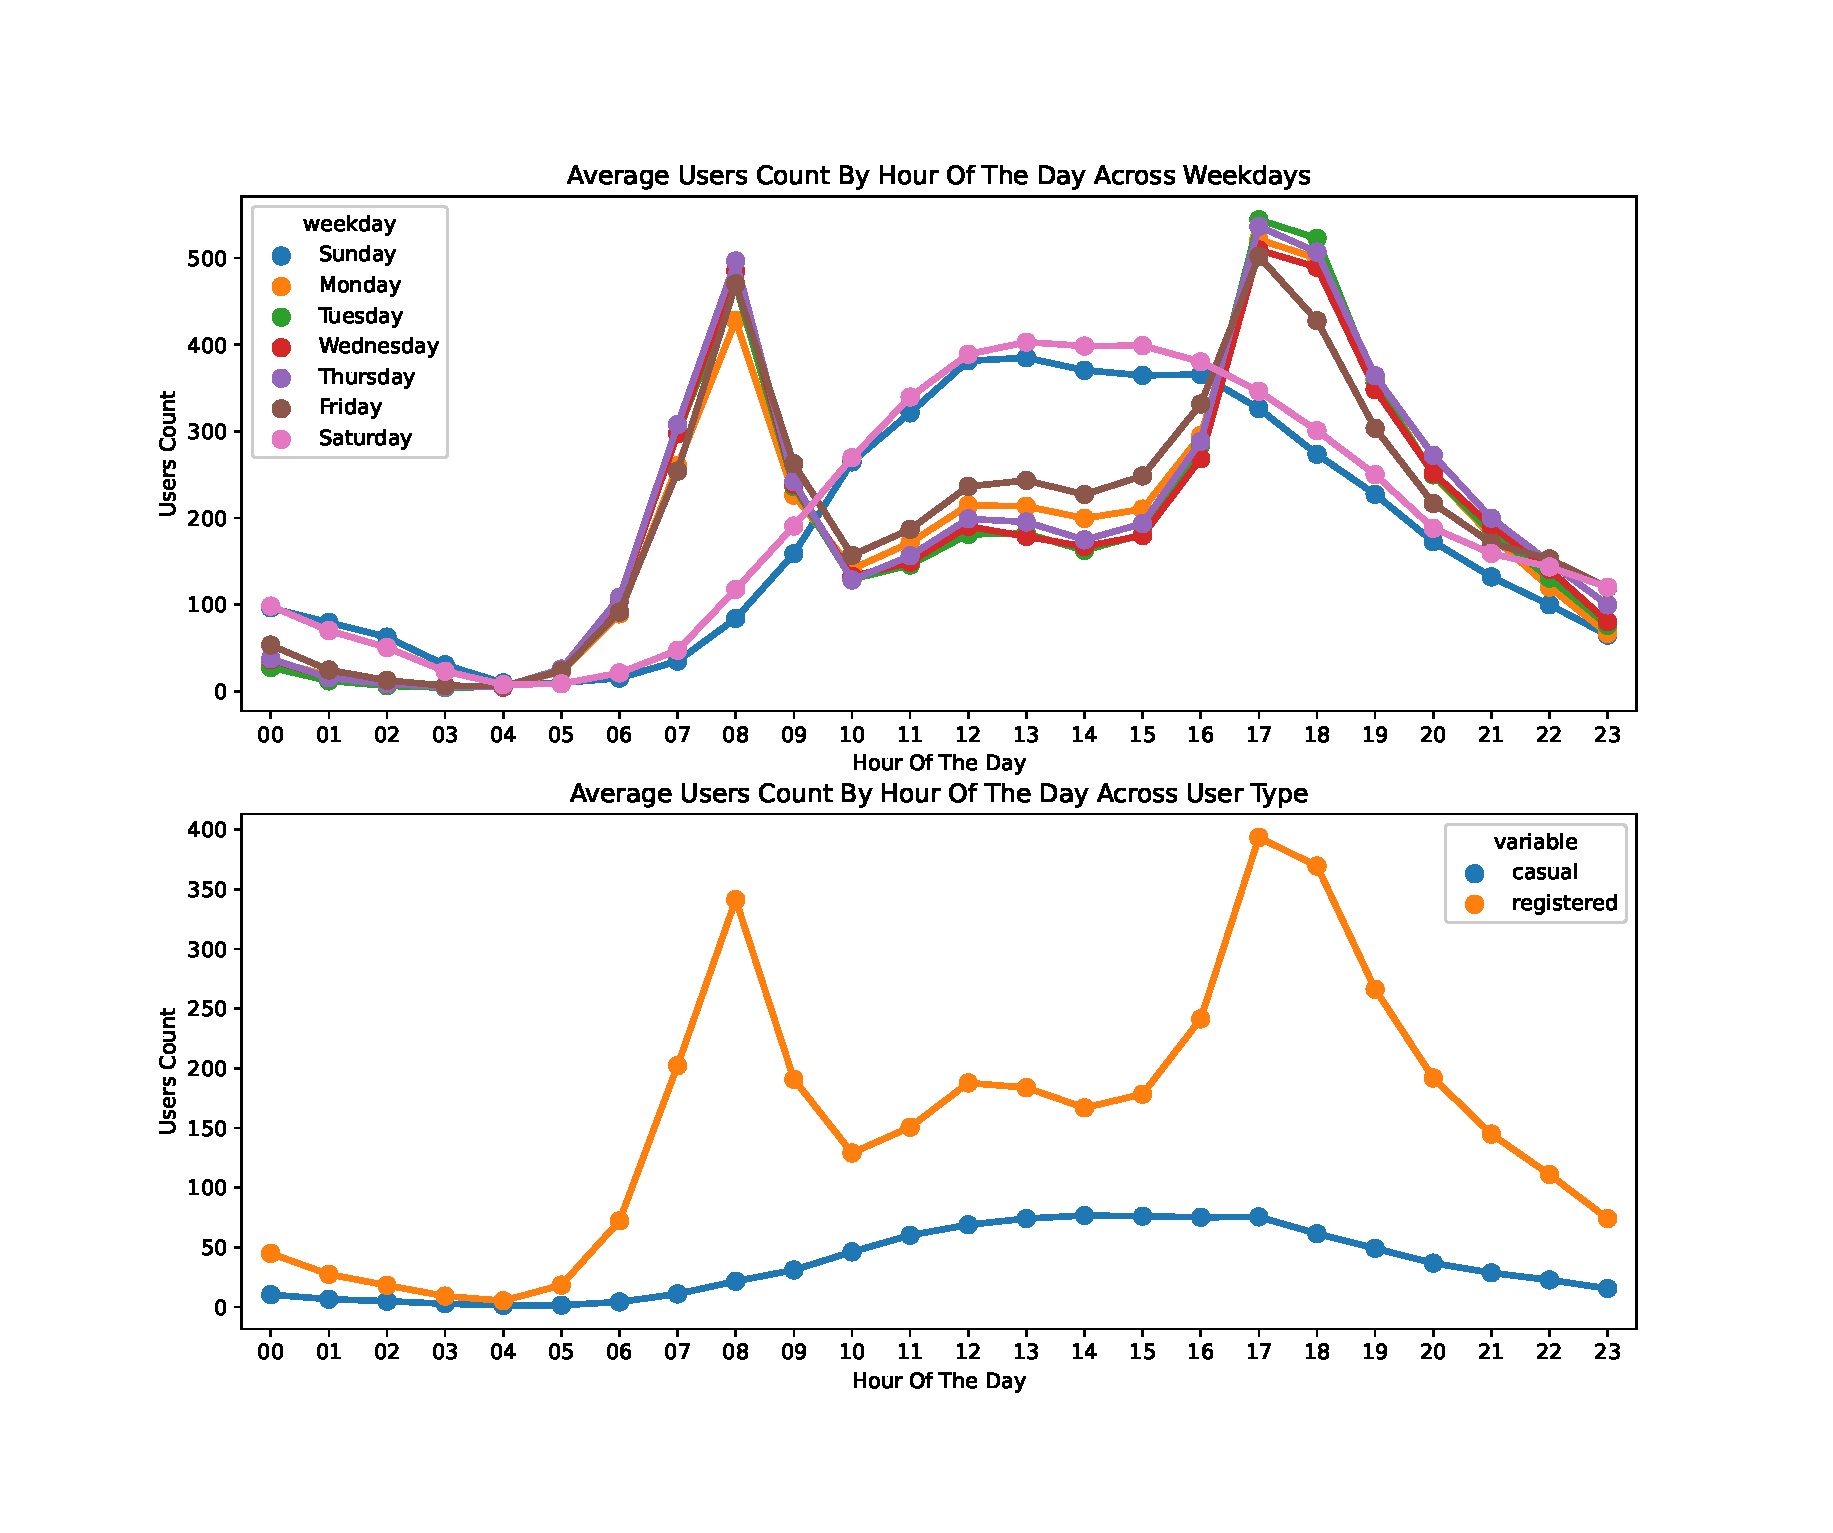
\includegraphics[width=.8\linewidth,height=.55\linewidth]{C:/FILP00report/picture/keshihua2.eps}
\end{center}
\end{slide}
%%
%%==========================================================================================


%%==========================================================================================
%%
\begin{slide}{Data Visualization Conclusion}
%Challenges (1)
\begin{itemize}
\item
It is quiet obvious that people tend to rent bike during summer season since it is really conducive to ride bike at that season.Therefore June, July and August has got relatively higher demand for bicycle.
\item
On weekdays more people tend to rent bicycle around 7AM-8AM and 5PM-6PM. As we mentioned earlier this can be attributed to regular school and office commuters.
\item
Above pattern is not observed on "Saturday" and "Sunday".More people tend to rent bicycle between 10AM and 4PM.
\item
The peak user count around 7AM-8AM and 5PM-6PM is purely contributed by registered user.
\end{itemize}

\end{slide}
%%
%%==========================================================================================


%%==========================================================================================
%%
\begin{slide}[toc=,bm=]{Visualizing Count Vs (windspeed,temp)}
\begin{itemize}
\item
windspeed \& temp
\end{itemize}
\vspace{-0.8cm}
\begin{center}
  \includegraphics[width=1.1\linewidth,height=.5\linewidth]{C:/FILP00report/picture/keshihua3.eps}
\end{center}
\end{slide}
%%
%%==========================================================================================


%%==========================================================================================
%%
\begin{slide}[toc=,bm=]{Data Visualization Conclusion}
\begin{itemize}
\item
The greater the wind speed, the less the frequency of use, there are also abnormal values of the average value.
\item
Suitable temperature range is about 20-30℃.
\end{itemize}
\end{slide}
%%
%%==========================================================================================

\section{Model}

%%==========================================================================================
\begin{slide}[toc=,bm=]{Train Model}
\begin{itemize}
\item
Linear Regression Model
After training the model, perform correlation analysis with the predicted data to obtain the linear regression value of RMSLE:0.977995978355
\item
Regularization Model - Ridge
\item
Regularization Model - Lasso
\end{itemize}
\end{slide}


%%
%%==========================================================================================

\begin{slide}[toc=,bm=]{Ensemble Models}
\begin{itemize}
\item
Ensemble Models - Random Forest
\item
Ensemble Model - Gradient Boost
\item
TO compare the distribution of train and test results. More or less the distribution of train and test looks identical.
\end{itemize}
\begin{center}
  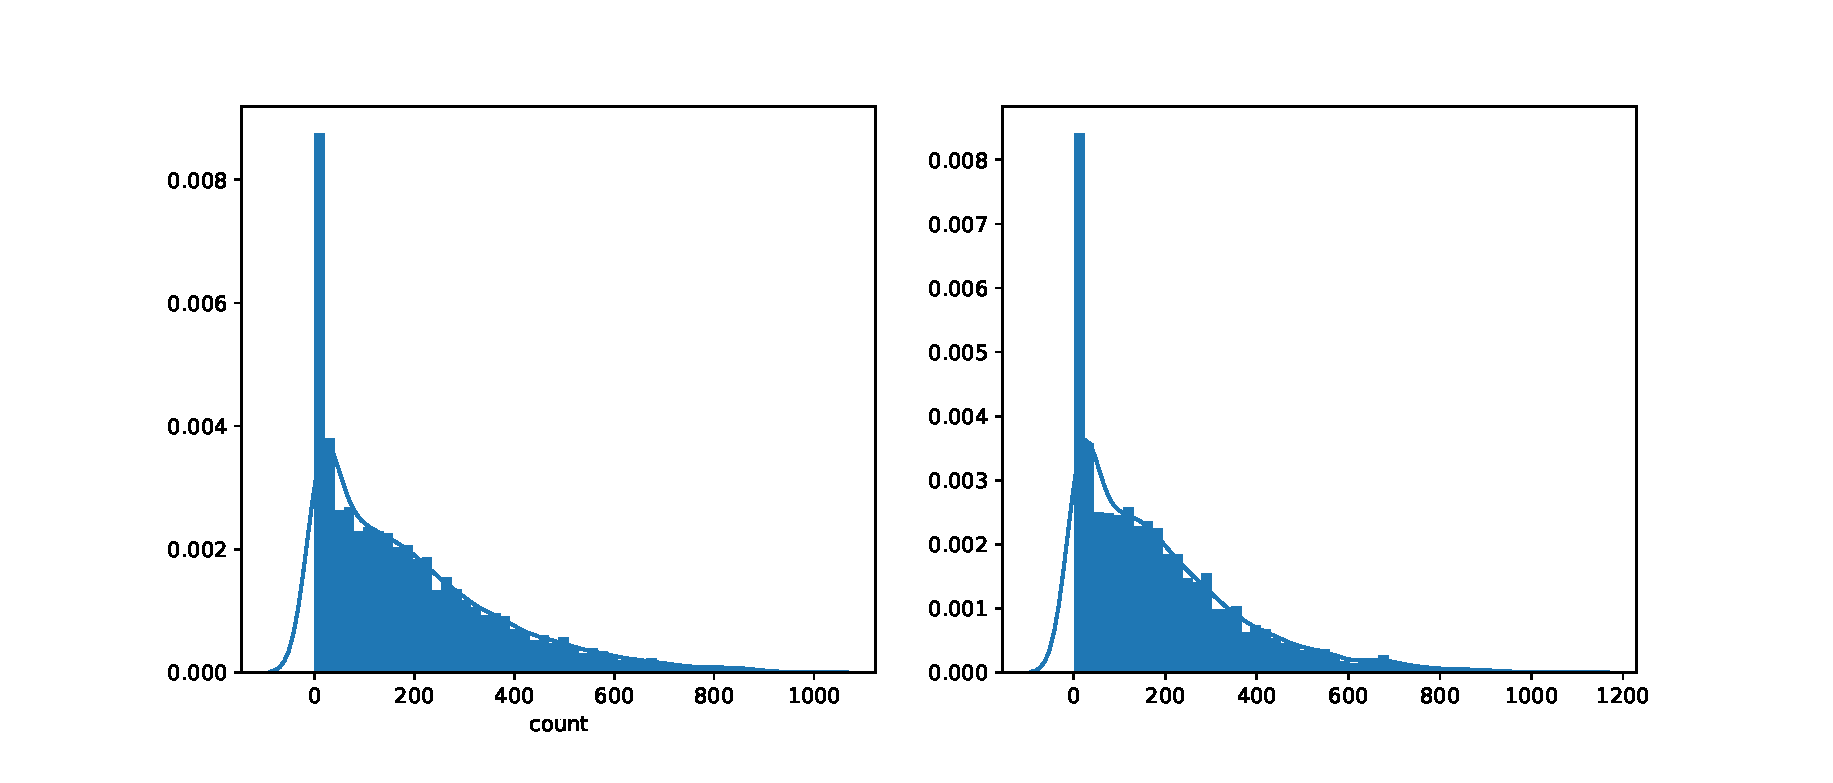
\includegraphics[width=.9\linewidth,height=.4\linewidth]{C:/FILP00report/picture/ending.eps}
\end{center}
\end{slide}
%%=========================================================================================
%%
\section{Thanks}

\end{document}

\endinput
